\documentclass{beamer}
\usepackage{pgfplots}
\usepackage{fontspec} 
\usepackage{langsci-optional}
% \usepackage{lsp-makros}
\useoutertheme{lsp}

\usepackage{lsptitle}

\def\two@digits#1{\ifnum#1<10 0\fi\number#1}
\def\mytoday{\two@digits{\number\day}.\two@digits{\number\month}.\number\year}


\usepackage{xspace,multicol}
\newcommand{\latex}{\LaTeX\xspace}
\usepackage{tikz}


\newcounter{lastpagemainpart}
\footnotesep0pt
\renewcommand{\footnoterule}{}
\usefootnotetemplate{
  \noindent
  \insertfootnotemark\insertfootnotetext}

\let\beamerfn=\footnote
\renewcommand{\footnote}[1]{%
\let\oldfnsize=\footnotesize%
\let\footnotesize=\tiny%
\beamerfn<\thebeamerpauses->{#1}%
\let\footnotesize=\oldfnsize}


\date{\mbox{2018-09-04, HIRMEOS Workshop, SUB Göttingen}}
% \newline HIRMEOS Workshop: Entity-Fishing for Digital Humanities and Scholarly Publishing, SLUB Göttingen}

\usepackage{eurosym}  
 
\renewcommand{\centerline}[1]{\hfill#1\hfill\hfill\mbox{}}


\title{Retrieving entities from publications in linguistics}%: Glottolog and Concepticon}
\institute{Language Science Press}
\author[LangSci]{Sebastian Nordhoff}



\begin{document}
\lspbeamertitle

\frame{
\frametitle{Outline}
\tableofcontents
}

\section{Linguistics}
\frame{
\frametitle{Linguistics}
\begin{itemize}
 \item  ca.\ 25,000 linguists worldwide
 \item  both monographs and articles 
 \item  rather long publication cycles 
 \item  less output than for instance biology
 \begin{itemize}
  \item possibility to keep track
 \end{itemize}
 \item  less sifting 
\end{itemize}
}
       
       
\frame{
\frametitle{How do linguists search for literature?}
\begin{itemize}
 \item For a domain you have little expertise of, how do you find relevant literature?
\end{itemize}

  \begin{tikzpicture}
    \begin{axis}[  
	axis lines*=left, 
        width  = .6\textwidth,
	height = \textheight,
%     	nodes near coords, 
	ytick=data,
	x tick label style={},  
	xmin=0,
	xbar=-2pt,
	bar width= 7pt,
	symbolic y coords={
	Researchgate,
	Ethnologue,
	WALS, 
	Personal collection, 
	Harald Hammarström, 
	Academia.edu,
	Mailing list, 
	Wikipedia,
	University library,
	Google Scholar,
	Glottolog,
	Personal contact
	},
	]
	\addplot+[lsRichGreen!80!black,fill=lsRichGreen] plot coordinates {
	    ( 2          ,Researchgate)
	    ( 2            ,Ethnologue)
	    ( 3                  ,WALS)
	    ( 3    ,Harald Hammarström)
	    ( 3          ,Academia.edu)
	    ( 3          ,Mailing list)
	    ( 3   ,Personal collection)
	    ( 4             ,Wikipedia)
	    ( 6    ,University library)
	    ( 7             ,Glottolog)
	    ( 7        ,Google Scholar)
	    ( 12     ,Personal contact)
	}; 
    \end{axis} 
  \end{tikzpicture} 
  
 {\tiny question asked on list \textit{Linguistic Typology} on 2018-08-29, no predefined answers\\[-.5em] n=18, multiple answers possible}
}
       
       
       
       
\section[LangSci]{Language Science Press}
\frame{
  \frametitle{Language Science Press}
  \begin{itemize}
  \item start 2014;  75 books; 22 series  
  \end{itemize}
  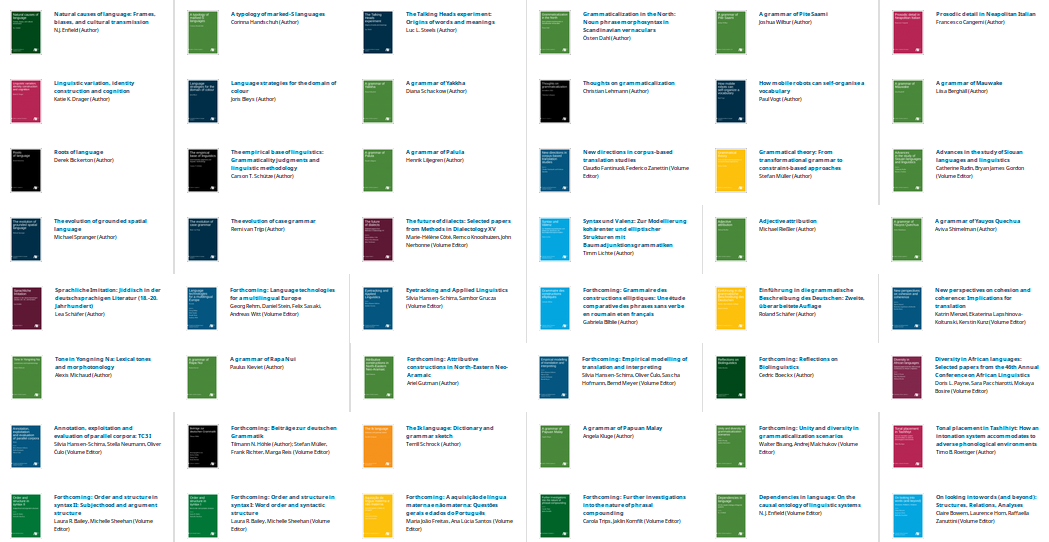
\includegraphics[height=.9\textheight]{catalog.png}
}

\frame{
\frametitle{Language Science Press}
\begin{itemize}
 \item   Available      formats for books
 \begin{itemize}
  \item pdf
  \item tex
  \item bib
 \end{itemize}             
 \item Indexes in books
 \begin{itemize}
  \item Language index
  \item Subject index 
  \item Name index
 \end{itemize} 
 \begin{itemize}
  \item Indexes are a discovery tool, similar to NERD.
 \end{itemize}
\end{itemize}
}
 

\frame{
\frametitle{\raggedright Bootstrapping index with sketchengine}
\begin{itemize}
 \item A recent book on film subtitles and eyetracking had the following index candidates generated by sketchengine
\end{itemize}
{\footnotesize
\begin{tabularx}{\textwidth}{XX}
image composition  \newline                
eye tracking       \newline           
speaking direction         \newline         
typographic identity     \newline             
fixation duration        \newline          
audiovisual translation  \newline                
aesthetic experience     \newline             
title area               \newline   
film material            \newline      
speaker identification   \newline               
film title               \newline   
natural focus            \newline      
text element             \newline     
image track              \newline    
information intake       \newline
graphical translation     \newline            
&
title placement           \newline      
bottom-centre area        \newline         
typographic film          \newline       
german image              \newline   
split attention           \newline      
gaze behaviour            \newline     
reading speed             \newline    
film identity             \newline    
typographic film identity \newline                
tracking research         \newline        
first fixation            \newline     
additional language       \newline          
narrative text            \newline     
eye tracking research     \newline            
visual attention          \newline       
individual placement      \newline   
\end{tabularx}
}
}

             
\section{NERD and linguistics}
\frame{
\frametitle{NERD and linguistics} 

\includegraphics[height=.4\textheight]{hirmeoslogo.jpg}
}

\frame{
\frametitle{Goals}
\begin{itemize}
 \item         higher level goals of text and data mining:
 \begin{itemize}
  \item provide better tools for exploration: \\
  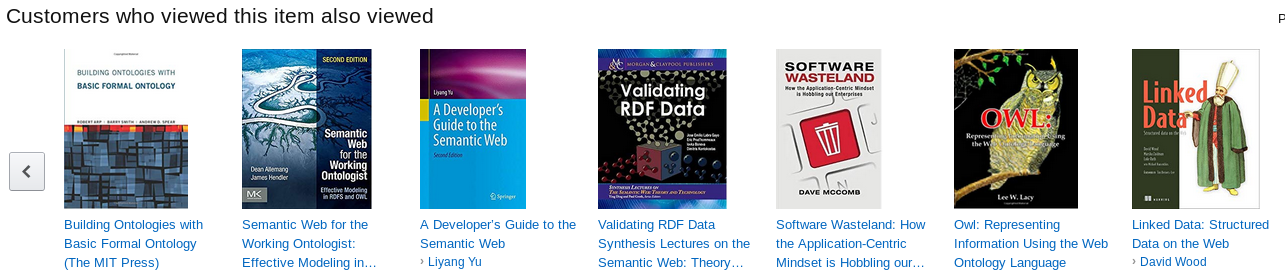
\includegraphics[height=2cm]{alsoviewed.png}
  \item automated reasoning:
  \begin{itemize}
   \item gene $\longleftrightarrow$ ~protein 
   \item ~\hphantom{gene $\longleftrightarrow$ }protein $\longleftrightarrow$ disease
   \item gene $\longleftrightarrow$ ~protein $\longleftrightarrow$ disease
  \end{itemize}
 \end{itemize}          
\end{itemize}
}

\frame{
\frametitle{Goals}
\begin{itemize} 
 \item  stated goals (Hirmeos):
 \begin{enumerate}
  \item   enhance discoverability
  \item   aggregation (word clouds)
  \item   generate collections 
  \item   highlighting
 \end{enumerate}           
\end{itemize}
}

\frame{
\frametitle{Relevant knowledge bases}
\begin{itemize}
 \item The following knowledge bases can be seen as resources for disambiguation

\begin{itemize}
 \item         
            \textbf{authority} (= Name Index)
            \begin{itemize}
             \item GND
             \item ORCID
            \end{itemize}
\item       \textbf{languoids} [languages, dialects, families] (= Language Index)
\begin{itemize}
 \item Glottolog
\end{itemize}

\item \textbf{concepts} (= Subject Index)
\begin{itemize}
 \item GOLD
 \item concepticon
\end{itemize}           
\end{itemize}
\end{itemize}
}

 
\frame{
\frametitle{Keywords}
\begin{itemize}
 \item Several platforms have fields for ``keywords'' (OMP, Zenodo)
\end{itemize}

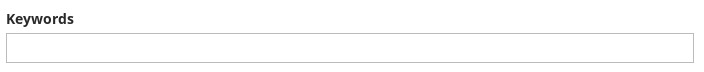
\includegraphics[width=.6\textwidth]{ompkeywords.png}
\begin{itemize}
 \item But should I really enter strings there?
 \end{itemize}

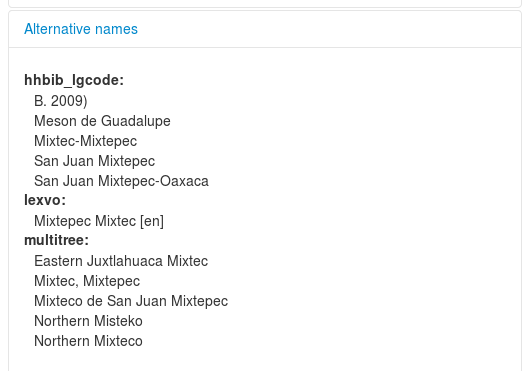
\includegraphics[height=.7\textheight]{mixtec-names.png}
}

\frame{
\frametitle{Person names}

\begin{columns}
  \begin{column}{4cm}
 
\includegraphics[height=\textheight]{saussure-cover.png}
  \end{column}
  \begin{column}{5cm}
    \begin{itemize}
      \item    GND
      \item ORCID
    \end{itemize}
  \end{column}
\end{columns}
}
        

 

\frame{
\frametitle{Language names: Glottolog}
\begin{itemize}
 \item        \textit{A grammar of   Komnzo}\\
 \noindent\hspace*{-1cm}
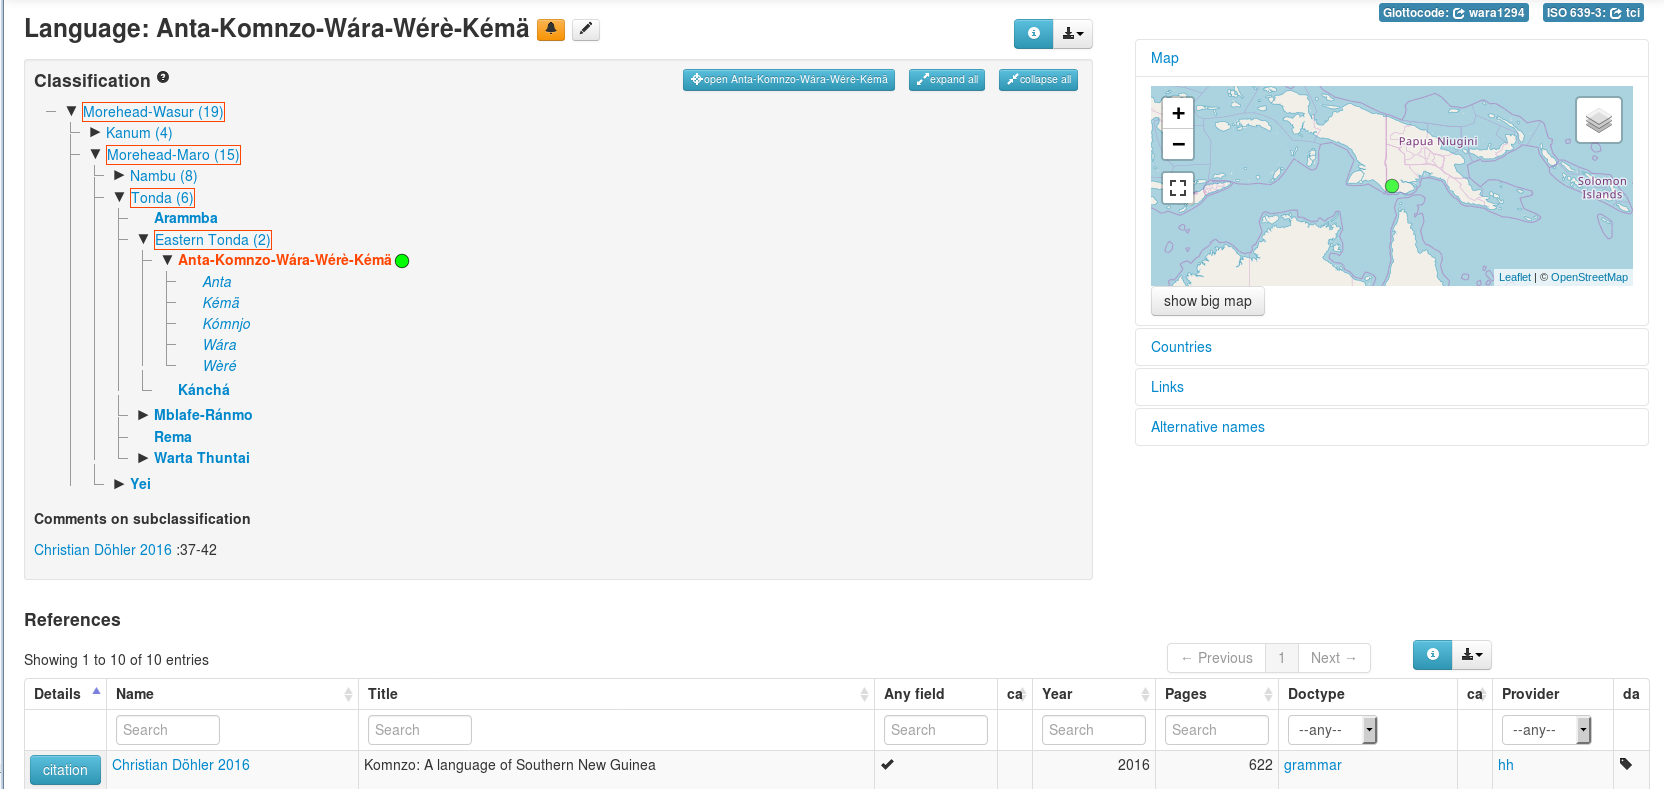
\includegraphics[width=1\textwidth]{komnzo-glottolog.png}\\ 
\end{itemize}
}
 
\frame{
\frametitle{Linguistic concepts}
\begin{itemize}
 \item          cross-linguistic categories don't exist\pause
 \item          cross-linguistic categories don't exist\pause
 \item          cross-linguistic categories don't exist\pause
 \item something called ``dative'' in language X cannot be equated with something called ``dative'' in language Y
 \begin{itemize}
  \item General Ontology for Linguistic Description (GOLD) tried and failed 
 \end{itemize}
\end{itemize}
}

\frame{
\frametitle{Inallative as ``cross-linguistic category''}
\begin{itemize}
 \item inallative
\end{itemize} 
\vspace*{-1cm}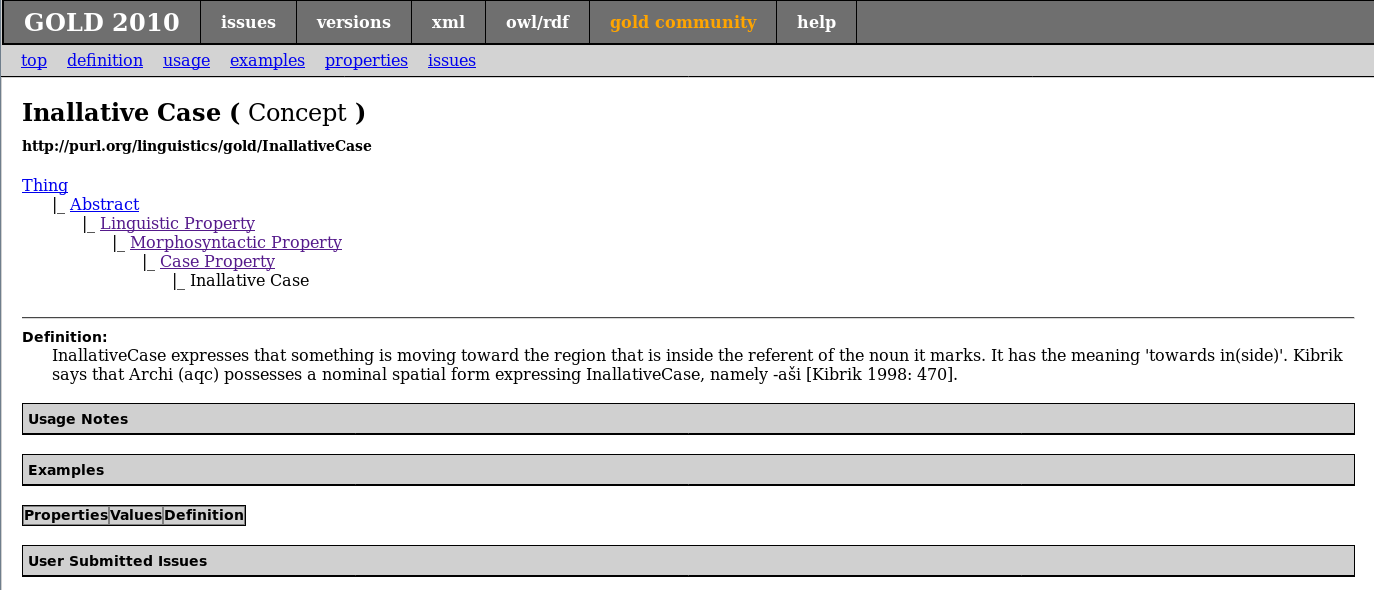
\includegraphics[height=.8\textheight]{inallative.png}\\ 
}
 
\frame{
\frametitle{What have the Romans ever done for us?} 
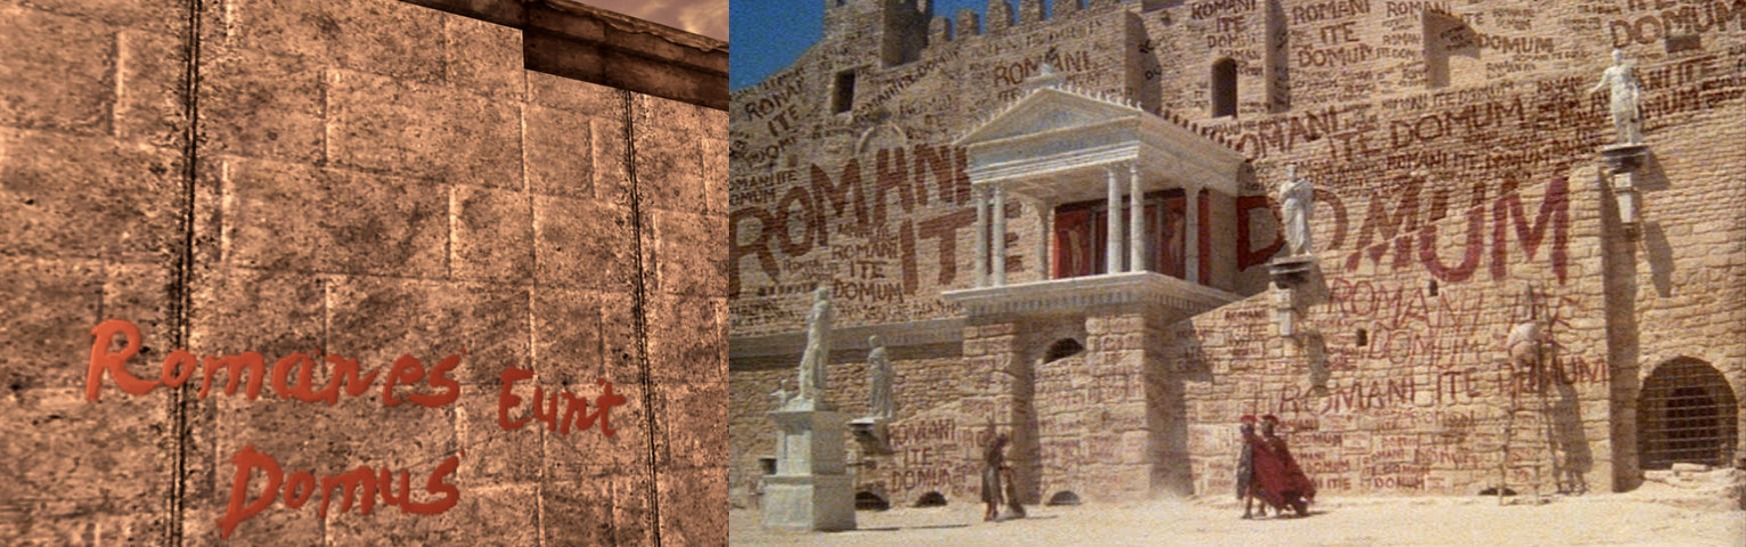
\includegraphics[width=\textwidth]{romaneseuntdomus.jpg} 
\begin{itemize}
 \item Is there an ``inallative'' in \textit{Romani ite domu\textbf{m}}?
 \item Is there an ``inallative'' in \textit{\textbf{au} foyer}?
 \item Is there an ``inallative'' in \textit{\textbf{t}huis}?
\end{itemize}
\begin{itemize}
 \item Can you equate the usages in the three examples?
 \item take-home-message: it's complicated, and automated\\ reasoning will not work. 
\end{itemize}


}
 

\section{Testing NERD}
\frame{
\frametitle{Testing NERD}\begin{columns}
  \begin{column}{4cm}
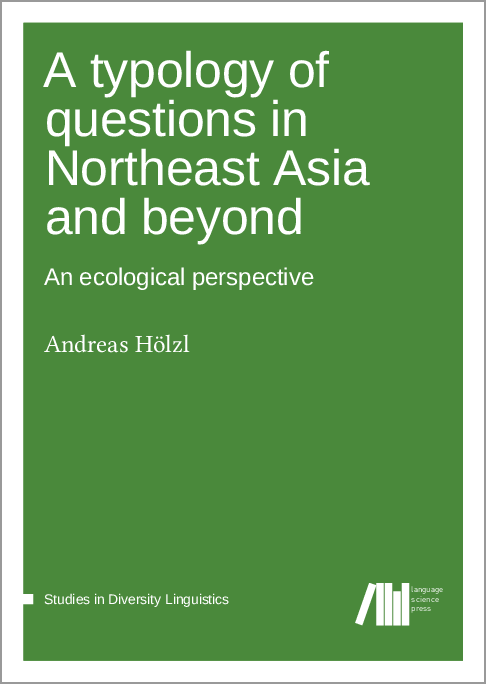
\includegraphics[height=\textheight]{hoelzl.png}
  \end{column}
  \begin{column}{5cm}
    \begin{itemize}
      \item \textit{A typology of questions in Northeast Asia and beyond}
      \item  Book chosen as the most recent publication 
      \item Variety of countries, languages, ethnic groups, concepts, etc.     
      \item 546 pages
    \end{itemize}
    \begin{itemize}
     \item NERD running on local machine 
    \end{itemize}

  \end{column}
\end{columns}

}

 

\frame{
\frametitle{Test section: Mongolic}
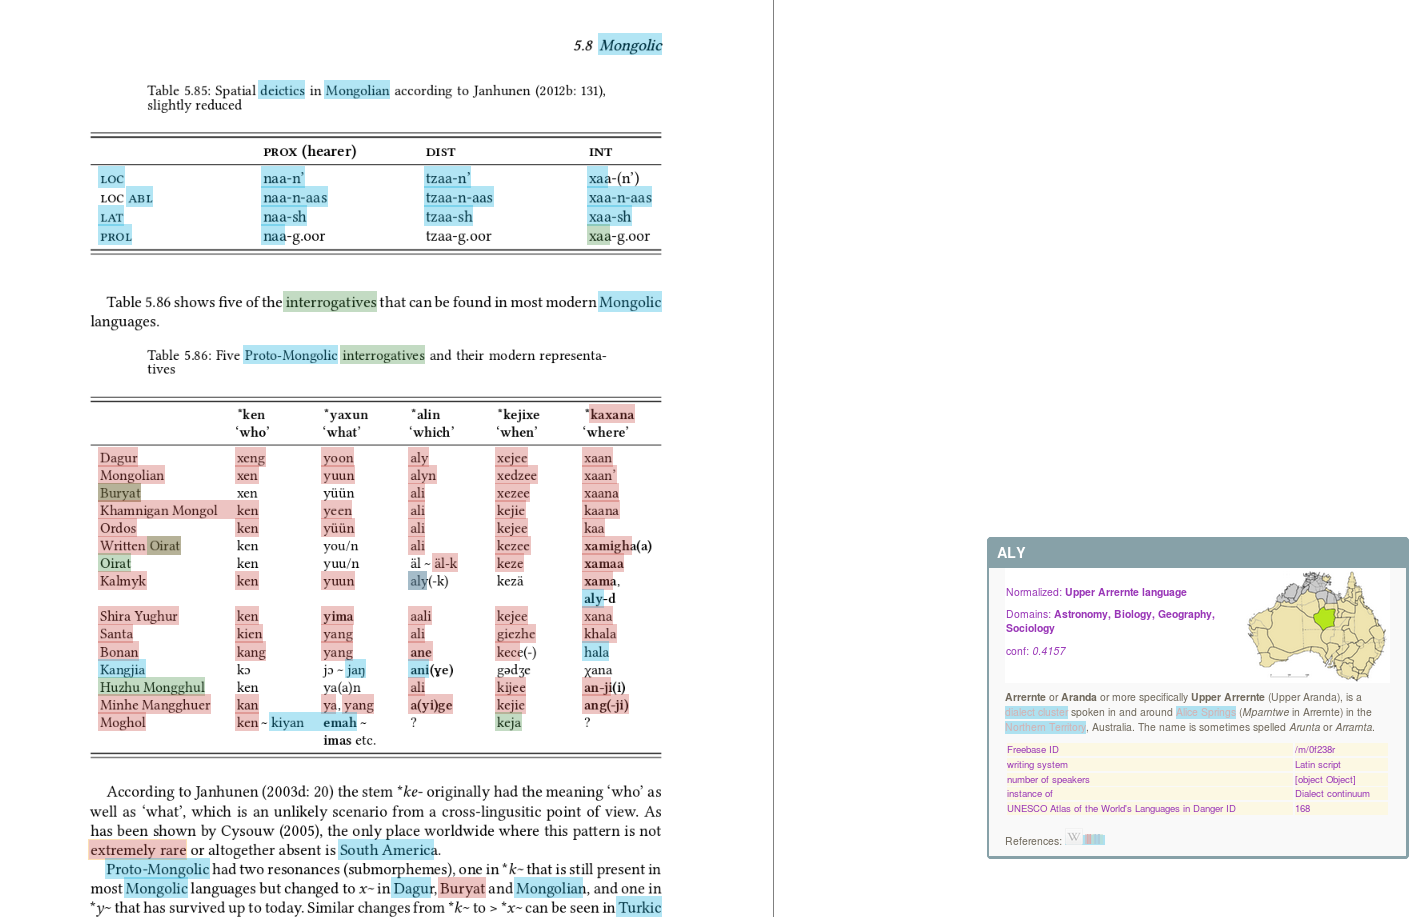
\includegraphics[height=\textheight]{mongolic.png}
}

\frame{
\frametitle{Results}
\begin{itemize}
 \item NERD retrieved some pretty specialized concepts
 \begin{itemize}
  \item Recall is good
 \end{itemize}
 \item NERD also retrieved a lot of irrelevant concepts (``South America'') or lookalikes (business names, radio stations)
 \item NERD was rather aggressive and colored whole pages.
 \item the system seems to have understood that the book is about linguistics and often selects a linguistic concept. However, sometimes, the concept chosen is off the mark (Australia). 
 \begin{itemize}
 \item Precision is low. 
 \end{itemize}
\end{itemize}
}

\frame{
\frametitle{Results}
\begin{itemize}
 \item Installation procedure was OK
 \item Loading the book in the browser worked out of the box
 \item Loading the book in the browser takes several minutes
\end{itemize}
}
 
\frame{
\frametitle{Questions from a publisher}
 \begin{itemize}
  \item in how far does NERD help the readers/authors? 
  \begin{itemize}
   \item Exploration/Discovery
      \begin{itemize}
	\item currently, discoverability of content via series, e.g. \textit{Contemporary African Linguistics}
	\item linguists seem to prefer personal/social interaction to automated recommender systems
      \end{itemize}
      \item Automated reasoning 
      \begin{itemize}
       \item limited potential given the fuzzy nature of cross-linguistic concepts
      \end{itemize} 
  \end{itemize}
\end{itemize}
}

\frame{
\frametitle{Goals (reprise)}
\begin{itemize} 
 \item  stated goals (Hirmeos):
 \begin{enumerate}
  \item   enhance discoverability: better than curated series?
  \item   aggregation (word clouds): better than index? 
  \item   generate collections: better than curated series? 
  \item   highlighting: is color a value in itself? 
 \end{enumerate}           
\end{itemize}
}


%\setcounter{framenumber}{\thelastpagemainpart}
\end{document}